
In this section, we evaluate the performance of the system for different workloads under different network and computing conditions. Specifically, we evaluate the offloading service handoff system by showing in what extent the total hand-off time and total transferred size are reduced.

In our experiment, we set up three migration scenarios\footnote{TODO:need a new design of experiments}: 
\begin{enumerate}
    \item VM-VM migration:
    Docker Hosts are two virtual machines on the same Desktop server. Docker containers are migrated from the Docker host to another Docker host.
    \item VM-Laptop-Ethernet: 
    One Docker host is a Virtual Machine on the Desktop server. Another Docker host  is a laptop connected via Ethernet. Docker containers are migrated from the virtual machine to the laptop via gigabit Ethernet connection\footnote{The actual network condition needs furthur confirmation}.
    \item VM-Laptop-Wireless:
    On Docker host is a virtual machine on the Desktop server, another is the same laptop as in 2). But the connection is changed. The laptop is connected by a wireless adapter. So the network changed to wireless connection.
\end{enumerate}

The desktop server is equipped with Intel$^{R}$ Core$^{TM}$ i3-6100 Processor (3.70GHz, 2 cores, 4 threads) and 16GB DDR4 memory. Two virtual machines are running with 2 vcpus and 4GB memory each.
The laptop is with Intel$^{R}$ Core$^{TM}$ Duo T6570 (2.2GHz, 2 cores) and 2GB DDR2 memory. Both the machines and virtual machines are running Ubuntu 16.04 LTS as the operating system.




TODO one large table here:

--------------------------------------

bandwidth/app   migration time / down time  /  FS size / Image size

5Mbps, 50ms

 \quad busybox
    
 \quad   face
    
  \quad  ...
    
10Mbps, 50ms

 \quad busybox
    
 \quad   face

  \quad  ...

15Mbps, 50ms

 \quad busybox
    
 \quad   face

  \quad  ...

25Mbps, 50ms

 \quad busybox
    
 \quad   face

  \quad  ...


30Mbps, 50ms

==========================================

% \begin{table}[!t]
% \centering

% \caption{Optimized using both layered images and compression with 5 Mbps bandwidth and 50 ms latency}
% \label{table_samehost_opt}


% % Some packages, such as MDW tools, offer better commands for making tables
% % than the plain LaTeX2e tabular which is used here.
% % \begin{tabular}{|l|l|l|l|l|l|}
% \begin{tabular}{|M{1.2cm}|M{0.9cm}|M{0.9cm}|M{1.3cm}|M{1.1cm}|
% % M{1.0cm}|
% }
% \hline
% Container & {Total time}  & {Down time} & { FS size} & { Mem size } 
% % & { Total Size }
% \\ \hline
% Busybox & $4.13s$ & $4.10s$ & $14KB$ & $29KB$ \\\hline
% OpenFace & $22.14 s$ & $22.00s$ & $100KB$ & $102.1MB$ \\\hline
% \end{tabular}
% \end{table}

% \begin{table}[!t]
% % increase table row spacing, adjust to taste
% % \renewcommand{\arraystretch}{2.5}
% % if using array.sty, it might be a good idea to tweak the value of
% % \extrarowheight as needed to properly center the text within the cells
% \centering

% \caption{Optimized using both layered images and compression with 5 Mbps bandwidth and 50 ms latency}
% \label{table_ethernet_opt}

% % Some packages, such as MDW tools, offer better commands for making tables
% % than the plain LaTeX2e tabular which is used here.
% % \begin{tabular}{|l|l|l|l|l|l|}
% \begin{tabular}{|M{1.2cm}|M{0.9cm}|M{0.9cm}|M{1.3cm}|M{1.1cm}|
% % M{1.0cm}|
% }
% \hline
% Container & {Total time}  & {Down time} & { FS size} & { Mem size } 
% % & { Total Size }
% \\ \hline 
% Busybox & $5.24s$ & $4.4s$ & $14KB$ & $29KB$ \\\hline
% OpenFace & $29.93s$ & $?s$ & $101KB$ & $102.1MB$ \\\hline
% \end{tabular}

% \end{table}


% \begin{table}[!t]
% % increase table row spacing, adjust to taste
% % \renewcommand{\arraystretch}{2.5}
% % if using array.sty, it might be a good idea to tweak the value of
% % \extrarowheight as needed to properly center the text within the cells
% \centering

% \caption{Optimized using both layered images and compression with 5 Mbps bandwidth and 50 ms latency}
% \label{table_wireless_opt}

% % Some packages, such as MDW tools, offer better commands for making tables
% % than the plain LaTeX2e tabular which is used here.
% % \begin{tabular}{|l|l|l|l|l|l|}
% \begin{tabular}{|M{1.2cm}|M{0.9cm}|M{0.9cm}|M{1.3cm}|M{1.1cm}|
% % M{1.0cm}|
% }
% \hline
% Container & {Total time}  & {Down time} & { FS size} & { Mem size } 
% % & { Total Size }
% \\ \hline
% Busybox & $7.12s$ & $6.80s$ & $14KB$ & $29KB$ \\\hline
% OpenFace & $60.23s$ & $60.20s$ & $101KB$ & $102.1MB$\\\hline
% \end{tabular}

% \end{table}



\begin{figure}[tb!]
    \centering
    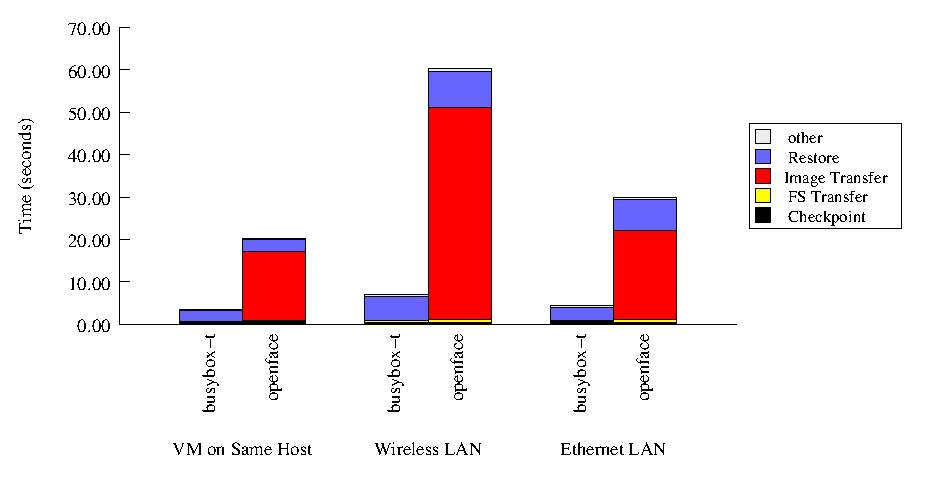
\includegraphics[width=\textwidth]{figure/test-tarssh.eps}
    \caption{Time of Container Migration Stages}
    \label{fig:timestage}
\end{figure}


TODO :
In order to make the result more comparable to others' work and avoid the effect of certain hardwares, we need to use Linux Traffic Control (tc\cite{tc} )  tool to control network traffic.
